\section{Aufgabe 17}
\textit{Fortsetzung Aufgabe 16.): Bestimmen Sie mit der in der VO besprochenen Methode
mit Iteration über die Länge der Keys unter Berechnung der Hamming Distanz (Slide
65, 2. Verfahren) die Länge des Keys in dem in Aufgabe 16.) realisierten short Key
XOR Verschlüsselungsverfahren.}\vspace*{1em}\newline
Wie bereits in der vorherigen Aufgabe beschrieben, wird ein Plaintext durch ein Short-Key-XOR-Verfahren verschlüsselt. Der verwendete Schlüssel sowie seine Länge sind dabei unbekannt. Gegeben ist lediglich der resultierende Ciphertext.
Zur Bestimmung der Schlüssellänge wird die durchschnittliche Hamming-Distanz benachbarter Blöcke des Ciphertexts analysiert. Hierfür werden unterschiedliche Blockgrößen getestet, wobei die jeweilige Blockgröße der vermuteten Schlüssellänge entspricht.
Die Funktion \verb|average_hamming_distance| berechnet die durchschnittliche Hamming-Distanz zweier aufeinanderfolgender Blöcke für einen gegebenen Ciphertext:
\begin{verbatim}
fn average_hamming_distance(cipher: &[u8], block_size: usize) -> f32 {
    let cipher_blocks = cipher.chunks(block_size).collect::<Vec<_>>();
    // ...
}
\end{verbatim}
Zunächst wird der Ciphertext mittels der \verb|chunks|-Methode in Blöcke der angegebenen Größe aufgeteilt. Anschließend wird die Hamming-Distanz aller benachbarten Blockpaare berechnet. Der Durchschnitt wird durch Division der Summe aller Distanzen durch die Anzahl der Blockpaare ermittelt:
\begin{verbatim}
let mut distances = Vec::new();
for block_pair in cipher_blocks.windows(2) {
    let a = block_pair[0];
    let b = block_pair[1];

    distances.push(hamming_distance(a, b) as f32);
}

distances.iter().sum() / distances.len() as f32
\end{verbatim}
Die Hamming-Distanz zweier Blöcke wird dabei folgendermaßen bestimmt: Die Bytes beider Blöcke werden paarweise XOR-verknüpft, und anschließend werden die Anzahl der Einsen (gesetzte Bits) im Ergebnis gezählt:
\begin{verbatim}
fn hamming_distance(a: &[u8], b: &[u8]) -> u32 {
    a.iter()
        .zip(b.iter())
        .map(|(x, y)| (x ^ y).count_ones())
        .sum::<u32>()
}
\end{verbatim}
Zur Bestimmung der tatsächlichen Schlüssellänge wird für alle potenziellen Schlüssellängen bis zur Hälfte der Ciphertextlänge die normierte durchschnittliche Hamming-Distanz berechnet. Schlüssellängen, die größer als die halbe Ciphertextlänge sind, werden ausgeschlossen, da dann keine ausreichende Anzahl an Blöcken zum Vergleich vorhanden ist. Die Normierung erfolgt durch Division der durchschnittlichen Hamming-Distanz durch die jeweilige Schlüssellänge:
\vspace*{1em}
\begin{verbatim}
let distances = (1..cipher.len() / 2)
    .map(|key_length|
        (key_length, 
        average_hamming_distance(cipher, key_length) / key_length as f32))
    .collect::<Vec<_>>();
\end{verbatim}

\subsection*{Ergebnisse}
Bei einem Experiment mit einer Schlüssellänge von $12$ Bytes und dem Plaintext:
\begin{quote}
"`Wird nicht ein kurzer repetitiver Schluessel verwendet sondern einer der
die gleiche Laenge aufweist wie der Plaintext, spricht man von OTP
Verschluesselung"',
\end{quote}
ergaben sich die Distanzen aus Abbildung \ref{fig:avg_hamming_distances}.
\begin{figure}[h]
    \centering
    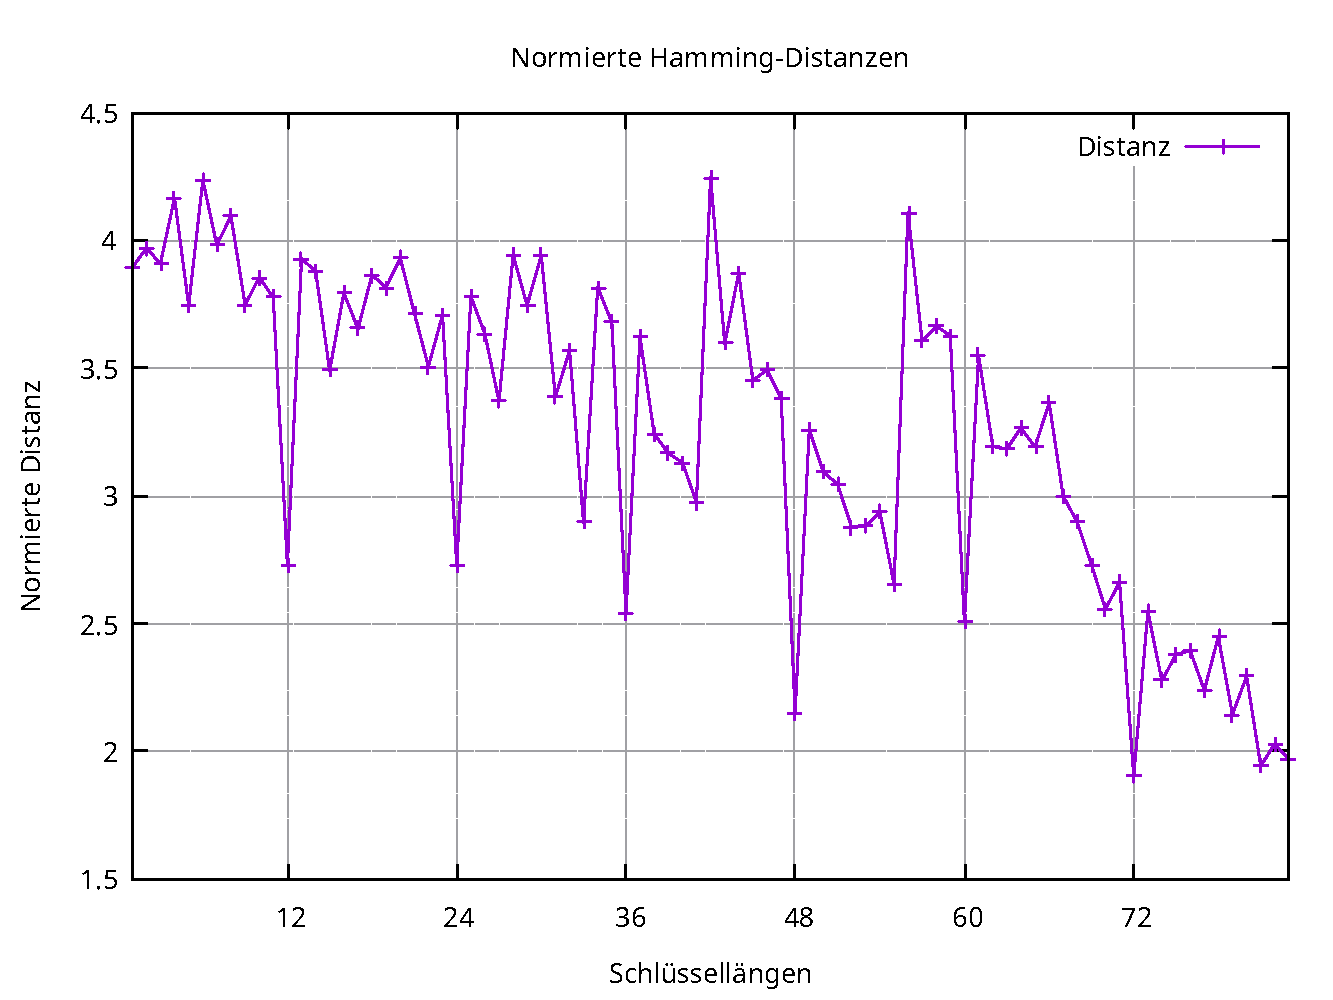
\includegraphics[width=0.8\textwidth]{img/plots/norm_hd_key_12.pdf}
    \caption{Normierte Hamming-Distanzen bei einer Schlüssellänge von 12 und einem 
    168 Zeichen langem Plaintext.}
    \label{fig:avg_hamming_distances}
\end{figure}
Je größer die geschätzte Schlüssellänge ist, desto niedriger wird die normierte 
Hamming-Distanz. Das liegt daran, dass mit einer zunehmenden Blockgrößer der
Durchschnitt der Hamming-Distanz an Aussagekraft verliert. Man kann aber deutliche
Minima bei $12$ und den Vielfachen erkennen. Dementsprechend würde man das erste
dieser Minima als Schlüssellänge verwenden.